\subsection*{Serie 01}
\subsubsection*{1.1.1}
Empirische Wahrscheinlichkeit für einen Gewinn:
\begin{align*}
h(A) = \frac{n_i}{n} = \frac{283789}{2300000} \approx 0.12339
\end{align*}
Wahrscheinlichkeit unter der Laplace-Annahme:
\begin{align*}
p(A) = \frac{m_i}{m} = \frac{3^3}{6^3} = \frac{27}{216} = 0.125
\end{align*}
\subsubsection*{1.1.2}
Wertebereiche der Zufallsvariablen:
\begin{align*}
X_{sum} & \in \{ 2, 3, 4, 5, 6,7,8,9,10,11,12\} \\
X_{min} & \in \{1, 2, 3, 4, 5, 6\}\\
X_{max} & \in \{1, 2, 3, 4, 5, 6\}\\
X_{diff1} & \in \{0, 1, 2, 3, 4, 5\}\\
X_{diff2} & \in \{-5, -4, -3, -2, -1, 0, 1, 2, 3, 4, 5\}
\end{align*}
Verteilung und Verteilungsfunktionen der Zufallsvariablen:\\

\newpage
\begin{center}
\begin{tabular}{|c|c|c|c|c|c|c|c|c|c|c|c|}
\hline 
$x_i$ & 2 & 3 & 4 & 5 & 6 & 7 & 8 & 9 & 10 & 11 & 12 \\ 
\hline 
$P(X_{sum}=x_i)$ & $\frac{1}{36}$ & $\frac{2}{36}$ & $\frac{3}{36}$ & $\frac{4}{36}$ & $\frac{5}{36}$ & $\frac{6}{36}$ & $\frac{5}{36}$ & $\frac{4}{36}$ & $\frac{3}{36}$ & $\frac{2}{36}$ & $\frac{1}{36}$ \\ 
\hline 
$A(x_i)$ & $\frac{1}{36}$ & $\frac{3}{36}$ & $\frac{6}{36}$ & $\frac{10}{36}$ & $\frac{15}{36}$ & $\frac{21}{26}$ & $\frac{36}{36}$ & $\frac{30}{36}$ & $\frac{33}{36}$ & $\frac{35}{36}$ & $\frac{36}{36}$\\ 
\hline 
\end{tabular}
\vspace{0.5cm}\\

\begin{tikzpicture}
\begin{axis}[
ybar,
symbolic x coords={2,3,4,5,6,7,8,9,10,11,12},
ylabel={$P(X_{sum}=x_i)$},
xtick=data]
\addplot table [x=x, y=y, col sep=comma] {serie_01/data/x_sum.txt};
\end{axis}
\end{tikzpicture}

\begin{tikzpicture}
\begin{axis}[
symbolic x coords={2,3,4,5,6,7,8,9,10,11,12},
ylabel={$A(x_i)$},
xtick=data]
\addplot+ [jump mark left] table [x=x, y=y, col sep=comma] {serie_01/data/x_sum_a.txt};
\end{axis}
\end{tikzpicture}
\end{center}

\newpage
\begin{center}
\begin{tabular}{|c|c|c|c|c|c|c|}
\hline 
$x_i$ & 1 & 2 & 3 & 4 & 5 & 6 \\ 
\hline 
$P(X_{min}=x_i)$ & $\frac{11}{36}$ & $\frac{9}{36}$ & $\frac{7}{36}$ & $\frac{5}{36}$ & $\frac{3}{36}$ & $\frac{1}{36}$ \\ 
\hline 
$A(x_i)$ & $\frac{11}{36}$ & $\frac{20}{36}$ & $\frac{27}{36}$ & $\frac{32}{36}$ & $\frac{35}{36}$ & $\frac{36}{36}$ \\ 
\hline 
\end{tabular} 
\vspace{0.5cm}\\

\begin{tikzpicture}
\begin{axis}[
ybar,
symbolic x coords={1,2,3,4,5,6},
ylabel={$P(X_{min}=x_i)$},
xtick=data]
\addplot table [x=x, y=y, col sep=comma] {serie_01/data/x_min.txt};
\end{axis}
\end{tikzpicture}

\begin{tikzpicture}
\begin{axis}[
symbolic x coords={1,2,3,4,5,6},
ylabel={$A(x_i)$},
xtick=data]
\addplot+ [jump mark left] table [x=x, y=y, col sep=comma] {serie_01/data/x_min_a.txt};
\end{axis}
\end{tikzpicture}
\end{center}

\newpage
\begin{center}
\begin{tabular}{|c|c|c|c|c|c|c|}
\hline 
$x_i$ & 1 & 2 & 3 & 4 & 5 & 6 \\ 
\hline 
$P(X_{max}=x_i)$ & $\frac{1}{36}$ & $\frac{3}{36}$ & $\frac{5}{36}$ & $\frac{7}{36}$ & $\frac{9}{36}$ & $\frac{11}{36}$ \\ 
\hline 
$A(x_i)$ & $\frac{1}{36}$ & $\frac{4}{36}$ & $\frac{9}{36}$ & $\frac{16}{36}$ & $\frac{25}{36}$ & $\frac{36}{36}$ \\ 
\hline 
\end{tabular} 
\vspace{0.5cm}\\

\begin{tikzpicture}
\begin{axis}[
ybar,
symbolic x coords={1,2,3,4,5,6},
ylabel={$P(X_{max}=x_i)$},
xtick=data]
\addplot table [x=x, y=y, col sep=comma] {serie_01/data/x_max.txt};
\end{axis}
\end{tikzpicture}

\begin{tikzpicture}
\begin{axis}[
symbolic x coords={1,2,3,4,5,6},
ylabel={$A(x_i)$},
xtick=data]
\addplot+ [jump mark left] table [x=x, y=y, col sep=comma] {serie_01/data/x_max_a.txt};
\end{axis}
\end{tikzpicture}
\end{center}

\newpage
\begin{center}
\begin{tabular}{|c|c|c|c|c|c|c|}
\hline 
$x_i$ & 0 & 1 & 2 & 3 & 4 & 5 \\ 
\hline 
$P(X_{diff1}=x_i)$ & $\frac{6}{36}$ & $\frac{10}{36}$ & $\frac{8}{36}$ & $\frac{6}{36}$ & $\frac{4}{36}$ & $\frac{2}{36}$ \\ 
\hline 
$A(x_i)$ & $\frac{6}{36}$ & $\frac{16}{36}$ & $\frac{24}{36}$ & $\frac{30}{36}$ & $\frac{34}{36}$ & $\frac{36}{36}$ \\ 
\hline 
\end{tabular} 
\vspace{0.5cm}\\

\begin{tikzpicture}
\begin{axis}[
ybar,
symbolic x coords={0,1,2,3,4,5},
ylabel={$P(X_{diff1}=x_i)$},
xtick=data]
\addplot table [x=x, y=y, col sep=comma] {serie_01/data/x_diff1.txt};
\end{axis}
\end{tikzpicture}

\begin{tikzpicture}
\begin{axis}[
symbolic x coords={0,1,2,3,4,5},
ylabel={$A(x_i)$},
xtick=data]
\addplot+ [jump mark left] table [x=x, y=y, col sep=comma] {serie_01/data/x_diff1_a.txt};
\end{axis}
\end{tikzpicture}
\end{center}

\newpage
\begin{center}
\begin{tabular}{|c|c|c|c|c|c|c|c|c|c|c|c|}
\hline 
$x_i$ & -5 & -4 & -3 & -2 & -1 & 0 & 1 & 2 & 3 & 4 & 5 \\ 
\hline 
$P(X_{diff2}=x_i)$ & $\frac{1}{36}$ & $\frac{2}{36}$ & $\frac{3}{36}$ & $\frac{4}{36}$ & $\frac{5}{36}$ & $\frac{6}{36}$ & $\frac{5}{36}$ & $\frac{4}{36}$ & $\frac{3}{36}$ & $\frac{2}{36}$ & $\frac{1}{36}$ \\ 
\hline 
$A(x_i)$ & $\frac{1}{36}$ & $\frac{3}{36}$ & $\frac{6}{36}$ & $\frac{10}{36}$ & $\frac{15}{36}$ & $\frac{21}{26}$ & $\frac{26}{36}$ & $\frac{30}{36}$ & $\frac{33}{36}$ & $\frac{35}{36}$ & $\frac{36}{36}$\\ 
\hline 
\end{tabular}
\vspace{0.5cm}\\

\begin{tikzpicture}
\begin{axis}[
ybar,
symbolic x coords={-5,-4,-3,-2,-1,0,1,2,3,4,5},
ylabel={$P(X_{diff2}=x_i)$},
xtick=data]
\addplot table [x=x, y=y, col sep=comma] {serie_01/data/x_diff2.txt};
\end{axis}
\end{tikzpicture}

\begin{tikzpicture}
\begin{axis}[
symbolic x coords={-5,-4,-3,-2,-1,0,1,2,3,4,5},
ylabel={$A(x_i)$},
xtick=data]
\addplot+ [jump mark left] table [x=x, y=y, col sep=comma] {serie_01/data/x_diff2_a.txt};
\end{axis}
\end{tikzpicture}  
\end{center}

\newpage
Kenngrößen der Zufallsvariablen:

\begin{center}
\begin{tabular}{|c|c|c|}
\hline 
Zufallsgröße & Erwartungswert & Varianz \\ 
\hline 
$X_{sum}$ & 7 & 5.833333333333333 \\ 
\hline 
$X_{min}$ & 2.5277777777777777 & 1.9714506172839503
 \\ 
\hline 
$X_{max}$ & 4.472222222222222 & 1.9714506172839508
 \\ 
\hline 
$X_{diff1}$ & 1.9444444444444446 & 2.052469135802469 \\ 
\hline 
$X_{diff2}$ & 0 & 5.833333333333334 \\ 
\hline 
\end{tabular} 
\end{center}

\subsubsection*{1.1.3}
Wertebereich der Zufallsvariable:
\begin{align*}
X \in \{i | i\in\mathbb{N}, 1 \leq i < \infty \}
\end{align*}
Diese Zufallsvariabe folgt der geometrischen Verteilung. Die Verteilungsfunktion ist
\begin{align*}
x(i) = (1-p)^{i-1} \cdot p
\end{align*}
mit $p=\frac{1}{6}$.
Für die Wahrscheinlichkeit, höchstens vier Würfe bis zum ersten Auftreten der Augenzahl 6, ergibt sich:
\begin{align*}
P(i \leq 4 ) = \sum_{k=1}^4 \frac{5}{6}^{k-1} \cdot \frac{1}{6} = 0.5177
\end{align*}
\subsubsection*{1.2.1}
Geometrische Verteilung $P_{geo}(X=n)=p (1-p)^{n}$ mit $p = 0.5$ :

\begin{center}
\begin{tikzpicture}
\begin{axis}[
ybar,
symbolic x coords={0,1,2,3,4,5,6,7,8,9,10},
ylabel={$P_{geo}(X)$},
xtick=data]
\addplot table [x=x, y=y, col sep=comma] {serie_01/data/geom.txt};
\end{axis}
\end{tikzpicture}
\end{center}
\vspace{0.5cm}
Exponentielle Verteilung $f_{\lambda}(x) = \begin{cases} \lambda e^{-\lambda x} & x \geq 0 \\ 0 & x < 0\end{cases}$ mit $\lambda = 2$ (grün), $\lambda = 1$ (blau) und $\lambda = 0.75$ (rot):
\begin{center}
\vspace{0.5cm}
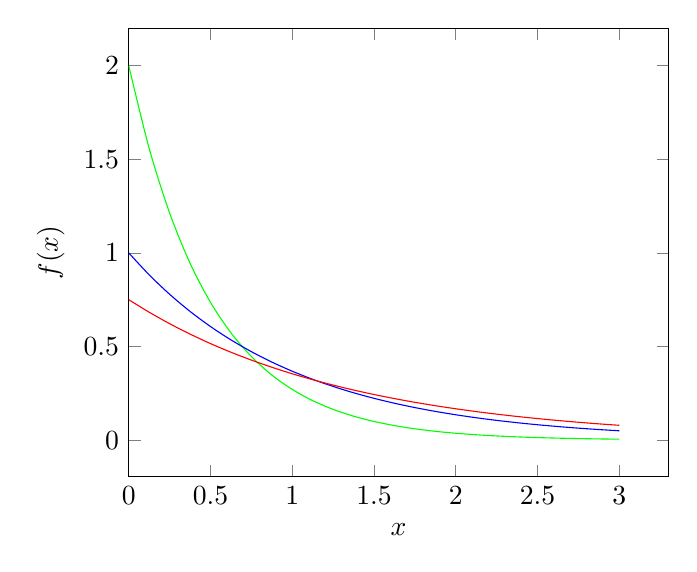
\begin{tikzpicture}
  \begin{axis}[ 
    xlabel=$x$,
    xmin=0,
    smooth,
    domain=0:3,
    ylabel={$f(x)$}
  ] 
    \addplot [color=green] {2*exp(-2*x)};
    \addplot [color=blue] {1*exp(-1*x)};
    \addplot [color=red] {0.75*exp(-0.75*x)};
  \end{axis}
\end{tikzpicture}
\end{center}
\subsubsection*{1.2.2}
Verteilungsdichtefunktion der geometrischen Verteilung für $p = 0.5$:
\begin{center}
\begin{tikzpicture}
\begin{axis}[
symbolic x coords={0,1,2,3,4,5,6,7,8,9,10},
ylabel={$P_{geo}(X)$},
xtick=data]
\addplot+ [jump mark left] table [x=x, y=y, col sep=comma] {serie_01/data/geom_a.txt};
\end{axis}
\end{tikzpicture}
\end{center}
Verteilungsdichtefunktion $F_\lambda$ der exponentiellen Verteilung mit $\lambda = 2$ (grün), $\lambda = 1$ (blau) und $\lambda = 0.75$ (rot):
\begin{equation*}
    F_{\lambda}(x) = \int_0^x \! f_\lambda(x) \, \mathrm{d}x = \begin{cases} 1 - e^{-\lambda x} & x \geq 0 \\ 0 & x < 0\end{cases} 
\end{equation*}

\vspace{0.5cm}
\begin{center}
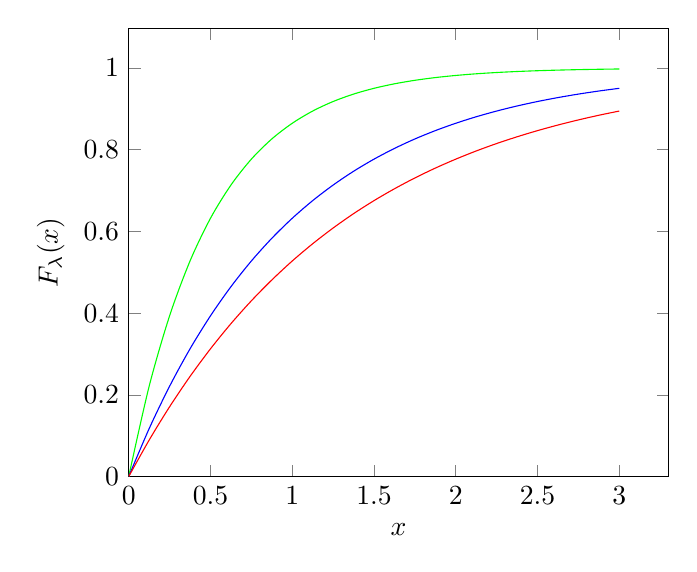
\begin{tikzpicture}
  \begin{axis}[ 
    xlabel=$x$,
    xmin=0,
    ymin=0,
    smooth,
    domain=0:3,
    ylabel={$F_\lambda(x)$}
  ] 
    \addplot [color=green] {1-(exp(-2*x))};
    \addplot [color=blue] {1-(exp(-1*x))};
    \addplot [color=red] {1-(exp(-0.75*x))};
  \end{axis}
\end{tikzpicture}
\end{center}
Unterschied: Die geometrische Verteilung ist diskret und die exponentielle Verteilung ist kontinuierlich. Dies liegt daran, dass die exponentielle Verteilung als Grenzfall aus der geometrischen Verteilung für $X$ herausgeht, wenn $p=1/n$ und $\frac{X}{n}$ für $n\xrightarrow{}\infty$ betrachtet wird.

\subsubsection*{1.2.3}
Wahrscheinlichkeit für $P(X\leq1)$ für die geometrische und exponentielle Verteilung:
\begin{align*}
P_{geo}(X \leq 1) & = 1-(1-p)^1 = p\\
P_{exp}(X \leq 1) & = 1-e^{-\lambda\cdot1} = 1-e^{-\lambda}
\end{align*}